%*******************************************************
% Chapter 0
%*******************************************************
\cleardoublepage
\chapter{Introduction}
\label{ch:chapter0:intro}
In the last ten years the robotics industry has increased year by year, and companies are seeing robotics as a decisive technology. According to ABI Research's \cite{abi-report} \enquote{State of the robotics market} report, during 2018 the total investment in robotics was about 4.000 million U\$S. Among these investments mobile robotics is recognized as one of the key trends, where the most important one is automated guided vehicles that move around contained environments, such as warehouses. \\

Within this context, \ac{UAV} systems are a growing industry, and although expectations were not fulfilled last years, they are considered as an emerging market. The cited report states that \enquote{the largest use case is undeniably for inspection and maintenance} \cite{abi-report}. Nevertheless, the current pandemic has open a door to innovation, and \ac{UAV}s are part of it \cite{eu-robotics-covid}. Leonardo, one of the biggest Italian companies in the market, has noticed that autonomous mobile systems will be important for its products in the near future, and for this reason, have launched an Open Innovation project aimed to \ac{UAV}s \cite{leonardo-drone-contest}.\\

The implementation presented in this work should be framed in the participation of the Politecnico di Milano Colibrì Team for the Leonardo Drone Contest. The team is a collaboration of the DEIB and the DAER departments, and had very positive results winning the first edition of the contest. % Unfortunately, the implementation presented in this work was not integrated by the time the competition took part. However, this work will remain for the next editions.\\
\section*{The contest}
The competition is composed of two phases. The map of the environment is developed during the first phase, while throughout the second phase the drone should follow a path of landmarks previously established. The drone should not have a GNSS signal nor can it be guided, this way, the drone is guaranteed to be fully autonomous, and as a result should complete both phases without any intervention.\\

The first phase the drone should map the environment, recognize the QR markers in the floor, avoid any obstacle and return to the initial position. During the second phase, and after the path of five landmarks is established, the drone should take off and land for at least five seconds in all the pre-defined markers in a specific order, and finally return to the initial position. The drone able to do the path in the right sequence is the winner of the competition. \\

The drone, as mentioned before, should not have any GNSS sensor nor LiDAR sensors, hence the localization and mapping algorithm should be based on visual information. The allowed sensors are inertial devices, like IMU or a magnetometer, range sensors, cameras and speed sensors, with the possibility of streaming capacity. \\

The indoor environment where the drone should move needs to have specific characteristics with obstacles and walls that delimit the space. Obstacles have at most three meters height with passages of at least one meter. An special QR marker of a size of one by one meter is disposed in the take-off area. The environment is 20 meters by 10 meters length, with the walls having a minimum of three meters height and made of net-like material. Furthermore, six poles are displaced in the following way: one per each corner and two in the middle axis, being each pole of different colors. The floor is a black, textured, pavement-like material. Obstacles are made of a high-visibility material, with a minimum volume of one cubic-meter.\\
\begin{figure}
    \centering
    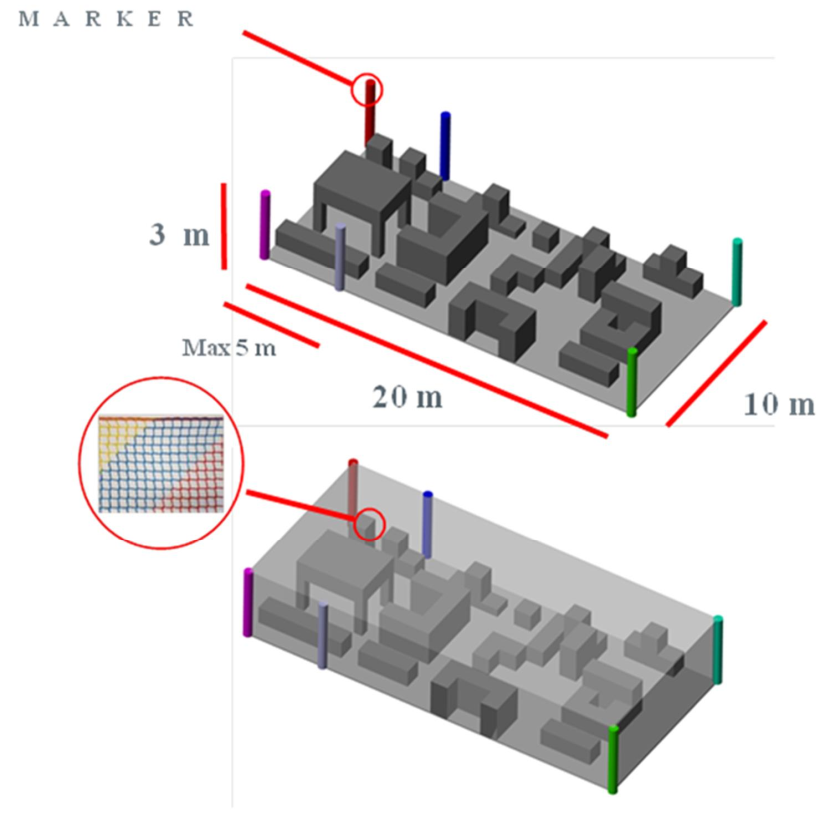
\includegraphics[width=0.6\textwidth]{Images/fig25-contest-env.png}
    \caption[Example of proposed environment]{Example of proposed environment for the Leonardo Drone Contest.}
    \label{fig:chapter0:contest-env}
\end{figure}

This work aims to shed some light on the importance of the usage of different landmarks in the environment, and how the implementation reacts on these different landmarks. Furthermore, it has the purpose to understand the importance of different implementation decisions included in the algorithm and how these decisions impacted on the results.
%\pagebreak
\section*{Road map}
The current work is divided in five chapters:
\begin{itemize}
    \item{\textbf{Chapter 2} introduces background information useful to completely understand the proposed implementation}
    \item{\textbf{Chapter 3} explains and comments the implementation in the context of the competition}
    \item{\textbf{Chapter 4} exposes the different experiments done in order to evaluate the implementation}
    \item{\textbf{Chapter 5} discusses over the results of the experiments and comments on possible future works and enhancements}
\end{itemize}
